\documentclass[12pt,a4paper]{article}

% Margins.
\setlength{\oddsidemargin}{0in}
\setlength{\evensidemargin}{0in}
\setlength{\headheight}{12pt}
\setlength{\headsep}{0pt}
\setlength{\topmargin}{-60pt}
\setlength{\textwidth}{6.5in}
\setlength{\textheight}{10.75in}

\usepackage{amsmath}
\usepackage{float}
\usepackage{graphicx}
\usepackage[hyphens]{url}
\usepackage{hyperref}	% Clickable links to figures, references and urls.
\usepackage{datetime}
\usepackage{longtable}

% Links direct to top of figures.
\usepackage[all]{hypcap}

% Drawing.
\usepackage{pgf}
\usepackage{tikz}

% Listings for formatting code.
\usepackage{listings}
\usepackage{textcomp}
% General options.
\lstset{breaklines=true, basicstyle=\small\ttfamily, tabsize=4, numbers=left, stepnumber=1, frame=single, showstringspaces=false, upquote=true}
% C++ specific high-lighting. Comments are 50/50 shades of green/black and strings coloured with 60/40 red/black mixture.
\lstset{language=[ISO]C++, commentstyle=\color{green!50!black}, keywordstyle=\color{blue}, stringstyle=\color{red!60!black}}

%opening
\title{Electromagnetic Theory\\Class 03\\Scalar and Vector Product of Vectors}
\author{Attique Dawood}
\date{August 22, 2014\\[0.2cm] Last Modified: \today, \currenttime}
\begin{document}
\maketitle
\section{Announcements}
\begin{itemize}
\item Assignment \#01 available.
\end{itemize}
\section{Revision}
\begin{itemize}
\item Usage of rec() and pol().
\item Position and distance vectors.
\item Scalar and vector fields.
\end{itemize}
\section{Exam Guidelines}
\begin{itemize}
\item Bring your own calculator. You cannot share calculators during quiz or exam.
\item Don't start writing unless asked to do so.
\item Don't write anything after the `Stop writing!' call.
\item All of the above (in addition to talking) are classified as cheating.
\item Cheating in a quiz results in cancellation of quiz. Cheating in successive quizzes results in F grade. Cheating in exam also results in F grade.
\end{itemize}
\textbf{Warning:} The invigilator is not supposed to ascertain if you actually cheated or not. If you're breaking the rules you're cheating, even if you asked the next person for their name.
\section{Multiplication of Vectors (1.7S)}
Multiplication of two vectors, \textbf{A} and \textbf{B}, results in a scalar or vector. There are two ways of multiplying two vectors.
\begin{enumerate}
\item Scalar (or dot) product. Dot product is written as $\textbf{A}\cdot \textbf{B}$ and the result is a scalar.
\item Vector (or cross) product. Cross product is written as $\textbf{A}\times \textbf{B}$ and the result is a vector.
\end{enumerate}
\subsection{Scalar Product}
Scalar product of two vectors \textbf{A} and \textbf{B} is obtained by multiplying magnitudes of both vectors and taking the cosine of smaller angle between them.
\begin{equation}
\textbf{A}\cdot \textbf{B}=AB\cos\theta_{AB}
\end{equation}
In component form, $\textbf{A}=A_x\hat x+A_y\hat y+A_z\hat z$ and $\textbf{B}=B_x\hat x+B_y\hat y+B_z\hat z$. Scalar product is then
\begin{equation}
\textbf{A}\cdot \textbf{B}=A_xB_x+A_yB_y+A_zB_z
\end{equation}
\begin{itemize}
\item[i.] Scalar product is commutative
\begin{equation*}
\textbf{A}\cdot \textbf{B}=\textbf{B}\cdot \textbf{A}
\end{equation*}
\item[ii.] Scalar product is distributive
\begin{equation*}
\textbf{A}\cdot (\textbf{B}+\textbf{C})=\textbf{A}\cdot \textbf{B}+\textbf{A}\cdot \textbf{C}
\end{equation*}
\item[iii.] Scalar product of a vector with itself gives the square of magnitude
\begin{equation*}
\textbf{A}\cdot \textbf{A}=|\textbf{A}|=A^2
\end{equation*}
\item[iv.] Scalar product of two unit vectors is 1 if they're same otherwise 0.
\begin{equation*}
\begin{split}
&\hat x\cdot\hat y=\hat y\cdot\hat z=\hat z\cdot\hat x=0\\
&\hat x\cdot\hat x=\hat y\cdot\hat y=\hat z\cdot\hat z=1
\end{split}
\end{equation*}
\end{itemize}
Two vectors are said to be \textit{orthogonal} (or perpendicular) to each other if their dot product is 0 as in the case of unit vector $\hat x$, $\hat y$ and $\hat z$. One way of understanding scalar product is to think of scalar product as a measure of how much two vectors are aligned with each other.
\section{Components of a Vector and Projections (1.8S)}
Scalar product is useful in finding vector projections and components along a certain direction. Given two vectors \textbf{A} and \textbf{B}, the \textit{vector component} of \textbf{A} along \textbf{B} is written as $\textbf{A}_B$ and is given by
\begin{equation}
\textbf{A}_B=(\textbf{A}\cdot \hat{a}_B)\hat{a}_B
\end{equation}
The \textit{scalar component} of \textbf{A} along \textbf{B} is simply
\begin{equation}
A_B=\textbf{A}\cdot \hat{a}_B
\end{equation}
This is illustrated in figure \ref{Scalar-vector-projections} taken from \cite[Figure 1.10, page 16]{Sadiku}.
\begin{figure}[H]
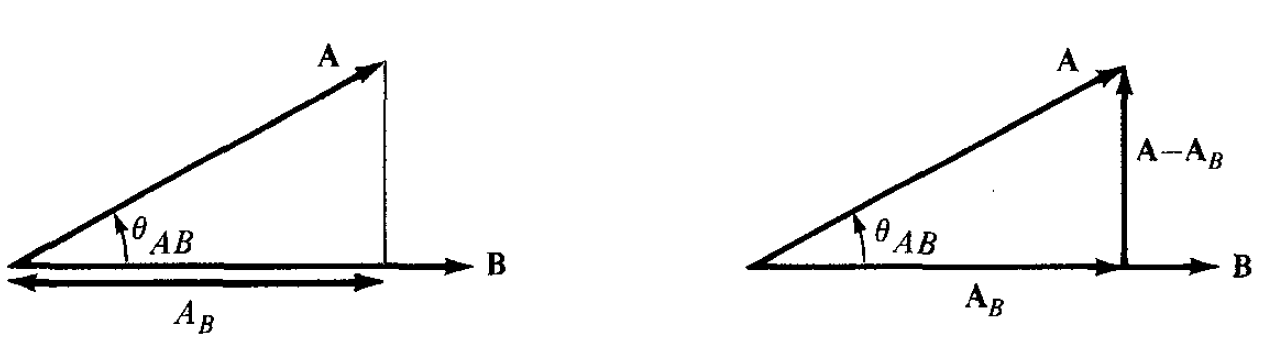
\includegraphics[scale=0.48]{Figure1-10S.png}
\caption{Scalar and vector projection of \textbf{A} along \textbf{B} \cite[Figure 1.10, page 16]{Sadiku}}
\label{Scalar-vector-projections}
\end{figure}
With respect to vector \textbf{B} we can think of vector \textbf{A} having two components, one that is along (or parallel to) \textbf{B}, $\textbf{A}_{B_\parallel}$; and another which is perpendicular (or orthogonal) to \textbf{B}, $\textbf{A}_{B_\perp}$. Also note that
\begin{equation}
\textbf{A}=\textbf{A}_{B_\parallel}+\textbf{A}_{B_\perp}
\end{equation}

\section{Exercises}
\noindent\textbf{Question 1:} Given $\textbf{A}=10\hat x-4\hat y+6\hat z$ and $\textbf{B}=2\hat x+\hat y$, find,
\begin{enumerate}
\item[(1)] The angle between \textbf{A} and \textbf{B}.
\item[(2)] The scalar component of \textbf{A} along $\hat y$.
\item[(3)] The vector component of \textbf{A} along $\hat y$.
\item[(4)] The vector component of \textbf{A} perpendicular to $y$-axis (or $\hat y$).
\item[(5)] The vector components of \textbf{A} parallel and perpendicular to $\hat z$. Do they add up to \textbf{A}?
\item[(6)] $\textbf{A}_{B_\parallel}$ and $\textbf{A}_{B_\perp}$. You can tell your answer is correct if $\textbf{A}=\textbf{A}_{B_\parallel}+\textbf{A}_{B_\perp}$.
\end{enumerate}
\section{Multiplication of Vectors (1.7S)}
Multiplication of two vectors, \textbf{A} and \textbf{B}, results in a scalar or vector. There are two ways of multiplying two vectors.
\begin{enumerate}
\item Scalar (or dot) product. Dot product is written as $\textbf{A}\cdot \textbf{B}$ and the result is a scalar.
\item Vector (or cross) product. Cross product is written as $\textbf{A}\times \textbf{B}$ and the result is a vector.
\end{enumerate}
\subsection{Vector Product}
Vector product of two vectors \textbf{A} and \textbf{B} is a vector whose magnitude is the area of the parallelogram formed by \textbf{A} and \textbf{B} and direction is perpendicular to both \textbf{A} and \textbf{B}. The direction or resultant vector follows right--hand rule.
\begin{equation}
\textbf{A}\times \textbf{B}=AB\sin\theta_{AB}\hat n
\end{equation}
In component form, $\textbf{A}=A_x\hat x+A_y\hat y+A_z\hat z$ and $\textbf{B}=B_x\hat x+B_y\hat y+B_z\hat z$. Vector product is then
\begin{equation}
\textbf{A}\times \textbf{B}=\left| \begin{array}{ccc} \hat{x} & \hat{y} & \hat{z} \\ A_x & A_y & A_z\\ B_x & B_y & B_z \end{array} \right|.
\end{equation}
Or
\begin{equation}
\textbf{A}\times \textbf{B}=(A_yB_z-A_zB_y)\hat x+(A_zB_x-A_xB_z)\hat y+(A_xB_y-A_yB_x)\hat z.
\end{equation}
\begin{itemize}
\item[i.] Vector product is anti--commutative
\begin{equation*}
\textbf{A}\times \textbf{B}=-\textbf{B}\times \textbf{A}
\end{equation*}
\item[ii.] Vector product is distributive
\begin{equation*}
\textbf{A}\times (\textbf{B}+\textbf{C})=\textbf{A}\times \textbf{B}+\textbf{A}\times \textbf{C}
\end{equation*}
\item[iii.] Vector product of a vector with itself is 0
\begin{equation*}
\textbf{A}\times \textbf{A}=0
\end{equation*}
\item[iv.] Vector product standard unit vectors is given below
\begin{equation*}
\begin{split}
&\hat x\times\hat y=\hat z\\
&\hat y\times\hat z=\hat x\\
&\hat z\times\hat x=\hat y\\
&\hat x\times\hat x=\hat y\times\hat y=\hat z\times\hat z=0
\end{split}
\end{equation*}
\end{itemize}
Right--hand rule is illustrated in figure \ref{Right-hand-rule} taken from \cite[Figure 1.8, page 14]{Sadiku}.
\begin{figure}[H]
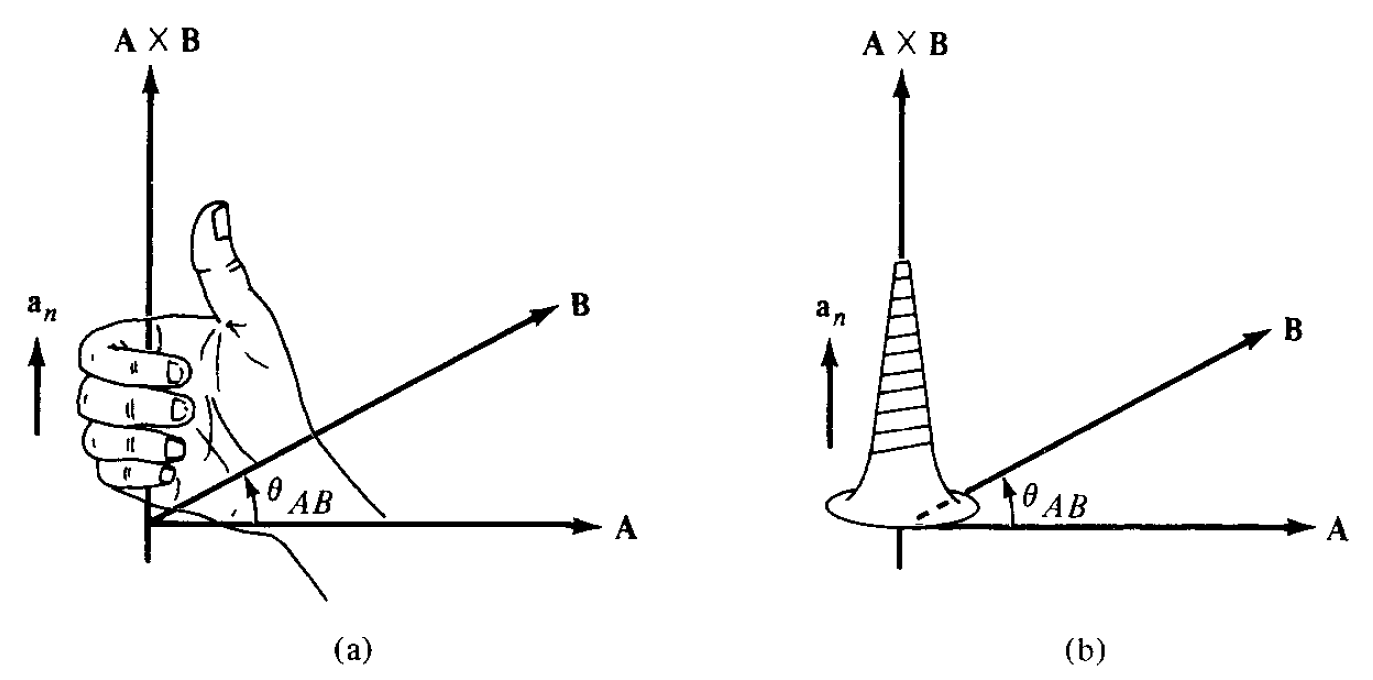
\includegraphics[scale=0.45]{Figure1-8S.png}
\caption{Right--hand rule for $\textbf{A}\times \textbf{B}$ \cite[Figure 1.8, page 14]{Sadiku}}
\label{Right-hand-rule}
\end{figure}
\subsection{Scalar Triple Product}
Given three vectors \textbf{A}, \textbf{B} and \textbf{C} the \textit{scalar triple product} is defined as
\begin{equation}
\textbf{A}\cdot (\textbf{B}\times \textbf{C})=\textbf{B}\cdot (\textbf{C}\times \textbf{A})=\textbf{C}\cdot (\textbf{A}\times \textbf{B})
\end{equation}
\begin{equation}
\textbf{A}\cdot (\textbf{B}\times \textbf{C})=\left| \begin{array}{ccc} A_x & A_y & A_z\\ B_x & B_y & B_z\\ C_x & C_y & C_z \end{array} \right|.
\end{equation}
\subsection{Vector Triple Product}
For three vectors \textbf{A}, \textbf{B} and \textbf{C} the \textit{vector triple product} is defined as
\begin{equation}
\textbf{A}\times (\textbf{B}\times \textbf{C})=\textbf{B}(\textbf{A}\cdot \textbf{C})-\textbf{C} (\textbf{A}\cdot \textbf{B})
\end{equation}

\section{Exercises}
\noindent\textbf{Question 1 (Example 1.5S):} Three field quantities are given by $\textbf{A}=2\hat x-\hat z$, $\textbf{B}=2\hat x-\hat y+2\hat z$ and $\textbf{C}=2\hat x-3\hat y+\hat z$ find,
\begin{enumerate}
\item[(1)] $(\textbf{A}+\textbf{B})\times(\textbf{A}-\textbf{B})$.
\item[(2)] $\textbf{B}\cdot \textbf{C}\times \textbf{A}$.
\item[(3)] $\textbf{A}\cdot \textbf{B}\times \textbf{C}$.
\item[(4)] $\textbf{A}\times(\textbf{B}\times \textbf{C})$.
\item[(5)] A unit vector perpendicular to both \textbf{B} and \textbf{C}.
\item[(6)] The vector component of \textbf{A} along \textbf{B}.
\end{enumerate}
\noindent\textbf{Question 2 (PE 1.5S):} Two field quantities are given by $\textbf{E}=3\hat y+4\hat z$ and $\textbf{F}=4\hat x-10\hat y+5\hat z$. Find,
\begin{enumerate}
\item[(1)] The component of \textbf{E} along \textbf{F}.
\item[(2)] Determine a unit vector perpendicular to both \textbf{E} and \textbf{F}.
\end{enumerate}
%\nocite{*}
\bibliographystyle{plain}
\bibliography{EMTRef}
\end{document}
